\chapter{Programmets brugergrænseflade}

I dette kapitel vil programmets grafiske brugergrænseflade blive beskrevet.

\section{Hovedvinduet} 
Hovedvinduet tilgås via vinduet \textbf{Login}, som åbner ved programstart. 

Der findes fire udgaver af hovedvinduet, forskellen mellem dem er, hvilke tabs der er aktive.
Hver tab indeholder forskellige funktioner, samlet set findes følgende tabs:
\begin{itemize}% Denne skulle måske relatere til tabel tab:permission
    \item Forside
    \item Undervisning
    \item Begivenheder
    \item Medlemmer
    \item Både.
\end{itemize}

Via hver af disse tabs, vil der være adgang til programmets forskellige funktionaliteter.
Programmet er lavet til at køre i opløsningen 1024x720 pixels.
Denne opløsning er valgt, da stort set alle computerskærme har en opløsning større end 1024x720 pixels \citep{resolutions}. 
Programmet har et lyst farveskema; med farverne lyseblå og hvid som primære farver.


\begin{center}
    \begin{figure}[H]
        \noindent{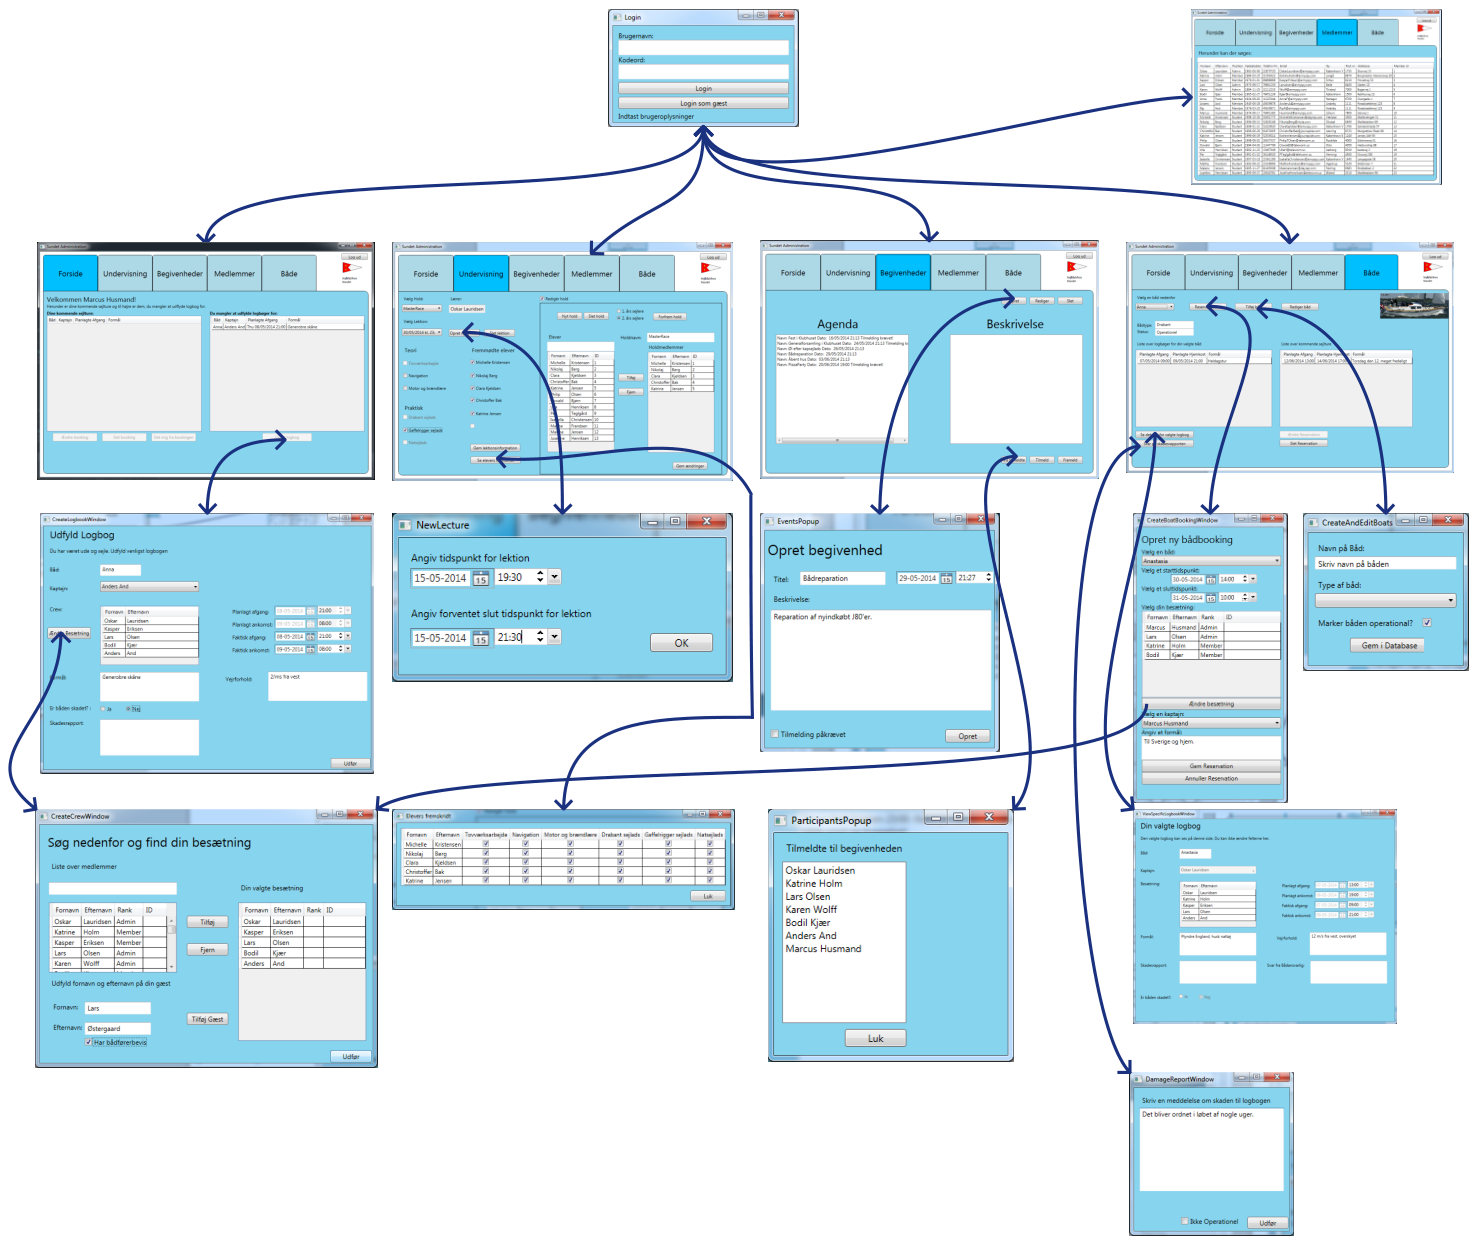
\includegraphics[width=0.9\textwidth]{UI/UI2.png}}
        \caption{Navigationsskema for programmet}
        \label{img:programNavigation}
        \vspace{-60pt}
    \end{figure}
\end{center}

%``'' == metoder/knapper/gui elementer
%textbf == vindue/tab/usercontrol
%textit= N/A

\section{Navigering i programmet}
På \myref{img:programNavigation} ses et navigationsdiagram for programmet.
Øverst er login-vinduet, herfra logger brugeren ind med sine login informationer, eller en gæst kan logge ind ved at trykke på knappen ``Login som gæst''. 
Brugeren ser nu hovedvinduet, hvilket er vinduet i midten med fem tabs i toppen.
Antallet af tabs varierer alt efter, hvilken position brugeren har i systemet, hvilket kan ses på \myref{tab:permissions}. 
Fra forside--tabben kan der navigeres til de andre tabs, som brugeren har adgang til.
Pilene illustrerer de dialogbokse, som brugeren kan åbne fra de forskellige tabs.
Dialogboksene åbnes ved at trykke på knapper inde i tabben, f.eks. under tabben \textbf{Både} kan dialogen \textbf{CreateBoatBookingWindow} åbnes ved at trykke på knappen ``Reserver Båden''. 
På samme måde åbnes de resterende dialoger ved tryk på knapper.
Flere steder i programmet anvendes de samme dialogvinduer, f.eks. fra tabben \textbf{Forside} findes en mulighed for at ændre på en reservation, hvilket åbner en mindre modificeret udgave af dialogen \textbf{CreateBoatBookingWindow}, hvorfra dialogen \textbf{CreateCrewWindow} også kan åbnes.
Desuden findes dialogen \textbf{CreateBoatBookingWindow} også fra tabben \textbf{Både}.
Dialogen \textbf{CreateLogBookWindow} åbnes fra tabben \textbf{Forside} mens en lignende dialog \textbf{ViewSpecificLogBookWindow} åbnes fra tabben \textbf{Både}.

% LaTeX tabel som viser alle brugerniveauer og deres muligheder efter login.
% http://bit.ly/1kToHZ3 to edit raw table
\begin{table}
    \centering
    \colorlet{shadecolor}{gray!40}
    \rowcolors{1}{white}{shadecolor}
    \begin{tabular}{l|llll}
    ~                        & Gæst & Medlem & Elev & Administrator \\ \hline
    Personlig forside        & ~    & \ding{51}      & \ding{51}    & \ding{51}             \\
    Se begivenheder          & \ding{51}    & \ding{51}      & \ding{51}    & \ding{51}             \\
    Tilmeld begivenheder     & ~    & \ding{51}      & \ding{51}    & \ding{51}             \\
    Opret begivenheder       & ~    & ~      & ~    & \ding{51}             \\
    Se sejlture              & \ding{51}    & \ding{51}      & \ding{51}    & \ding{51}             \\
    Opret sejltur            & ~    & \ding{51}      & \ding{51}    & \ding{51}             \\
    Se logbøger              & \ding{51}    & \ding{51}      & \ding{51}    & \ding{51}             \\
    Opret logbog             & ~    & \ding{51}      & \ding{51}    & \ding{51}             \\
    Svar på logbog           & ~    & ~      & ~    & \ding{51}             \\
    Se undervisningstimer    & ~    & ~      & \ding{51}    & \ding{51}             \\
    Opret undervisningstimer & ~    & ~      & ~    & \ding{51}             \\
    \end{tabular}
    \caption{Tabel over alle brugerniveauer og deres tilladte funktioner.}\label{tab:permissions}
\end{table}


\section{UserControls}
Der anvendes UserControls til at kode både brugergrænsefladen og den tilhørende Code-Behind.
Hver usercontrol kan ses på \myref{img:programNavigation}

\subsection{DateTimePicker}\label{subsec:DateTimePicker}

\begin{wrapfigure}{r}{0.5\textwidth}
    \label{img:DateTimePicker}
    \vspace{-20pt}
    \begin{center}
        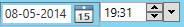
\includegraphics[width=0.48\textwidth]{Screenshots/DateTimePicker.png}
    \end{center}
    \vspace{-15pt}
    \caption{DateTimePicker}
    \vspace{-30pt}
\end{wrapfigure}

\textbf{Formål}: 
Denne UserControl er lavet, da der ikke fandtes en tilfredsstillende løsning, som gjorde det muligt at vælge både dato og tidspunkt i samme control. 
Det er ofte nødvendigt at vælge både dato og tidspunkt samtidigt i programmet. 

\textbf{BrugerGrænseflade}: 
Den består af en DatePicker og en TimePicker, som findes i extended WPF toolkit.

\textbf{Code-Behind}: 
Der er lavet en specifik getter og setter for UserControlen, som udnytter både controllens DatePicker og TimePicker.


\subsection{Forside}

\textbf{Formål}: 
Formålet med forsiden er at vise aktuel infomation på en overskuelig måde for brugeren.
Det er den første side i hovedvinduet, som man ser, med mindre man er gæst.
Fra forsiden kan man ændre og slette sine reservationer, samt starte oprettelsen af en logbog.

\textbf{Brugergrænseflade}: 
Brugergrænsefladen på forsiden består primært af to DataGrids: Det venstre DataGrid viser brugerens kommende sejlture, og det højre viser de sejlture brugeren mangler at udfylde logbøger for. 
Under dem er der knapper, som bliver aktive, efter en markering er udført ved at trykke på en af rækkerne i knappernes tilhørende DataGrid.

\textbf{Code-Behind}: 
For kun at vise de sejlture hvor personen, som er logget ind, deltager i anvendes der standard query operatorer. 
I listing \ref{fntpg-cb} er der et udsnit af koden, nærmere bestemt den del som vælger de korrekte sejlture.

Begge udtryk returnerer en IEnumerable, som derefter assignes som ItemsSource til hvert DataGrid.

\begin{lstlisting}[frame=single, caption=Forsidens Code-Behind, label=fntpg-cb]
// Sets the trips for the person currently logged in while only getting the ones in the future to the DataGrid ItemsSource
UpcommingTripsDataGrid.ItemsSource =
    sailTripList.Where(t => t.Crew.Select(p => p.PersonId).Contains(usrId))
        .Where(t => t.DepartureTime > DateTime.Now);
// Sets trips created by the current user which happened in the past while also missing a logbook, as the other DataGrids ItemsSource 
LogbookDataGrid.ItemsSource =
    sailTripList.Where(t => t.Captain.PersonId == usrId && t.ArrivalTime < DateTime.Now && t.Logbook == null);
\end{lstlisting}

\subsection{Boat}

\textbf{Formål:}
I tabben \textbf{Både}, finder man UserControllen \textbf{Boat}.
Her kan man få et overblik over hvilke både, der er til rådighed i sejlklubben inklusiv bådtype og status på de enkelte både.
Man kan også reservere en båd, se liste over logbøger for en valgt båd, svare på skadesrapporten og ligeledes se en liste over kommende reservationer. 

\textbf{Brugergrænseflade:}
Efter valg af båd opdateres de resterende elementer i UserControllen. 
Her kan der ses et DataGrid med udfyldte logbøger samt et andet DataGrid med kommende reservationer på båden.
Som administrator kan man også svare på logbogens skadesrapport.
Foruden disse funktionaliteter kan man også herinde reservere den valgte båd.
Desuden har administratorer mulighed for at tilføje og redigere både.

\textbf{Code-Behind:}
Den bagvedliggende kode henter data fra databasen og opdaterer de grafiske elementer med dataet.

\subsection{StudyTeacher}

\textbf{Formål:}
Denne UserControl bruges til give undervisere på sejlerskolen mulighed for at administrere skolehold og undervisningslektioner.

\textbf{Brugergrænseflade:}
Når der er valgt et hold, er der forskellige controls som opdateres.
Man kan se holdets underviser, elever og hvorvidt holdet er et 1. eller 2. års hold. 
Det er også muligt at se holdets lektioner, samt oprette og slette disse.
Når der trykkes på knappen ``Opret ny Lektion'', åbnes et nyt vindue, hvor man skal indtaste start- og sluttidspunkt, og trykke ok, for at afslutte sin oprettelse af lektionen.
Efter der er valgt en lektion, kan der afkrydses hvad der er lært på lektionen, samt hvilke elever der var fremmødte.
Ved tryk på knappen ``Se elevers fremskridt'' åbnes et vindue, hvor man kan se hvilke læringsområder, de enkelte elever har gennemført.
Når der laves et nyt hold, åbnes et vindue, hvor man blot indtaster det ønskede navn for holdet.
Der kan slettes og forfremmes hold, hvilket betyder de får et bådførerbevis.

\textbf{Code-Behind:}
Når der oprettes en lektion, bliver der reserveret den korrekte båd på det pågældende tidspunkt.
Når der forsøges at forfremme et hold, tjekker Code-Behinden, om eleverne har, lært alt det de skal og ændrer herefter eleverne fra StudentMember til SailClubMember og sætter deres BoatDriver property til \texttt{true}.

Der findes også en undervisnings UserControl for elever. 
Denne kan ikke interageres med, men viser blot hvilke læringsområde brugeren har lært, informationer om det hold de er på, samt hvornår deres næste lektion er planlagt.

\subsection{Event}
\textbf{Formål:}
UserControllen Event bruges til at se informationer om kommende begivenheder i sejlklubben, samt til at tilmelde sig begivenhederne. 
Hvis man er administrator, kan man også oprette nye begivenheder, redigere og slette eksisterende begivenheder.

\textbf{Brugergrænseflade:}
Brugergrænsefladen består af to ListBoxe og nogle knapper.
I den første ListBox bliver begivenheder vist med navn, dato og om hvorvidt der kræves tilmelding.
I den næste ListBox vises beskrivelsen af begivenheden, som opdateres, når der klikkes på en begivenhed i den førnævnte ListBox. 

\textbf{Code-Behind:}
Den bagvedliggende kode henter oprettede begivenheder fra persistenslaget. 
Ved oprettelse, redigering og sletning skrives ændringerne til persistenslaget. 
Ved tilmelding tilføjes personen, som er logget ind, til listen over tilmeldte personer.

\section{Vinduer}
Alle vinduer beskrevet i dette afsnit kan ses på \myref{img:programNavigation}. 
\subsection{Login}
 
\textbf{Formål}:
Vinduet \textbf{Login} har til formål at verificere en brugers identitet. 
Det er det første vindue brugeren ser, når programmet åbnes, og det åbner hovedvinduet efter succesfuldt login.
 
\textbf{Brugergrænseflade}:
Der er en TextBox til brugernavnet og en PasswordBox til kodeordet.
En PasswordBox er en TextBox, hvor hver af de indtastede karakterer vises som en sort prik, i stedet for de skrevne tegn, for at beskytte brugeren.
Knappen ``Login som gæst'' kræver ingen brugeroplysninger og åbner en let udgave af hovedvinduet, uden særlige tilladelser.
Til sidst er en TextBlock, som fortæller brugeren, hvad og hvis, der er skrevet noget forkert.

\textbf{Code-Behind}: \fxnote{Troels: Dette burde nok udvides bare lidt?}
Efter der trykkes på knappen ``Login'', verificeres infomationen som er indtastet.
TextBoxen, hvor brugernavnet indtastes, er case insensitive.
PasswordTextBoxen er case sensitive.
Hvis det er gyldigt, åbnes en passende udgave af hovedvinduet i hendhold til \myref{tab:permissions}.

\subsection{CreateBoatBookingWindow}
\textbf{Formål}: 
Dette vindue opretter eller ændrer en instans af RegularTrip, det vil sige en bådreservation. 

\textbf{Brugergrænseflade}: 
Først benyttes en ComboBox til at vælge hvilken båd, der skal reserveres.
Herefter anvendes UserControllen \textbf{DateTimePicker} til at vælge et start- og sluttidspunkt.
Der vises den nuværende besætning, samt muligheden for at ændre den ved at trykke på knappen ``Ændre Besætning'', som åbner \textbf{CreateCrewWindow}.
Når en besætning er valgt, kan der vælges en person ud fra besætningslisten, som har førerbevis, som kaptajn.
Til sidst er der en TextBox, hvori brugeren kan angive formålet med turen.

\textbf{Code-Behind}: 
I Code-Behinden er der to constructors. 
Den ene bruges til at oprette en ny reservation, den anden bruges når der skal ændres på en eksisterende reservation. 
Efter tryk på knappen ``Gem Reservation'', verificeres brugerens input fra alle de grafiske elementer i vinduet, og passende responsbeskeder gives, hvis noget er ugyldigt.

\subsection{CreateCrewWindow}

\textbf{Formål}: Dette vindue åbnes to steder i programmet: i \textbf{CreateLogbookWindow} og i \textbf{CreateBoatBookingWindow}. 
Det bruges, når der skal laves en besætning til en RegularTrip.  

\textbf{Brugergrænseflade}: 
Der er to DataGrids, som hver indeholder en liste. 
Listen til venstre består af SailClubMembers, som bliver hentet ind fra persistenslaget.
Listen til højre indeholder det Crew, som man er i gang med at udforme til enten RegularTrip eller Logbook. 
Der er også tilføjet TextBoxe, så man kan skrive navnet på en gæst, man tog med på sejlturen. 
Der er knapper, som tilføjer de forskellige personer til besætnings-listen. 
Øverst findes også et tekstfelt til at søge i listen over medlemmer. 
Når man har lavet sin liste, kan man trykke Udfør, for at komme tilbage til vinduet, der kaldte CreateCrewWindow.

\textbf{Code-Behind}: 
Der er blevet brugt en regular expression til at tjekke, om den string brugeren angiver i de to TextBoxe for gæstens navne, er gyldige. 
Det er blevet valgt, at man må bruge hele det danske alfabet samt mellemrum, så navne såsom: Lars Peter Østergaard, er mulige.
Derefter tilføjes personen til listen, der vises i DataGridet til højre, og til sidst kaldes RefreshDataGrid, som man kan se på \myref{RefreshDatagrid}.

Her modtages der et DataGrid, som skal have dets Itemssource opdateret, og en ICollection<Person>, som er det data, der skal sættes ind i DataGridet. 
Det gøres ved at assigne dets ItemsSource til null, og derefter assigne det tilbage til den ICollection, der blev sendt med. 
Der kan laves en tilsvarende metode, som opdaterer andre WPF-controls, for andre ItemsSources.

\begin{lstlisting}[frame=single, caption=Refresh Datagrid, label=RefreshDatagrid]
private void RefreshDatagrid(DataGrid Grid, ICollection<Person> list)
{
    Grid.ItemsSource = null;
    Grid.ItemsSource = list;
}
\end{lstlisting}

\subsection{CreateLogbookWindow}

\textbf{Formål}: 
Dette vindue bruges til at udfylde logbogen for en sejltur.

\textbf{Brugergrænseflade}:  
Når vinduet åbnes, indlæses der data fra den instans af RegularTrip, som logbogen udfyldes for, hvilket bliver sendt til vinduets constructor.
Som tidligere vinduer, bliver dataet afbilledet i de respektive grafiske elementer. 
De tomme felter skal udfyldes af brugeren.

\textbf{Code-Behind}: 
Code-Behinden verificerer dataet inden det gemmes i databasen.
Herudover sættes referencen til logbogen i det pågældende RegularTrip.

